
Für die Umsetzung der im Kapitel \ref{sec:Konzept} angesprochenen Ideen und
Eigenschaften wurde die Programmiersprache C++ verwendet. Als Entwicklungsumgebung kommt
Eclipse zum Einsatz. Zur Verbesserung der Teamarbeit und des Austausches
von Quellcode wurde ein Github Repository \footnote{www.github.com} angelegt,
welches über das Eclipse-Plugin EGit genutzt wurde. \newline Im Folgenden wird
im Detail auf die Art und Weise der Realisierung der beiden Top-Level-Module
\Code{Sender} und \Code{Receiver} eingegangen. Hierfür wurde eine flexible und
modulare Softwarearchitektur entwickelt, damit auf spätere Änderungen, neue Anforderungen
und erforderlichen Optimierungen flexible reagieren werden kann. Dies ist durch
das einfache Austauschen kompletter Module möglich.
Dafür wird ein objektorientiertes Design genutzt, womit Quellcoderedundanzen und damit
zahlreiche potentielle Programmierfehler vermieden werden konnten.
Weiterhin ist die Wiederverwendung einzelner Quellcodepassagen möglich.\newline
Damit die beiden Module in anderen Projekten einfach genutzt werden können,
wurde eine statische Library erstellt, welche über eine Schnittstelle die Funktionen
der beiden Module bereitstellt. In dieser Arbeit wurden nur die beiden
Datentypen Text und Sensorwerte integriert.

\section{Modulaufbau Sender}

Die Aufgabe des Moduls \Code{Sender} besteht darin, die aus vier Phasen
bestehende Verarbeitung der Daten aus \todo{LINK zur crop-arbeit} umzusetzen. In
\abbildung{BlockdiagrammSender} ist das Blockdiagramm des Moduls \Code{Sender}
darstellt.
Dies bietet eine Übersicht zu den Modulen und wie diese untereinander 
Kommunizieren. In der Grafik ist jedes Submodul durch ein M in der linken
oberen Ecke des Blockes gekennezeichnt. Ebenso ist die Schnittstellenklasse angegeben
und durch die Abkürzung IF (Interface) gekennzeichnet. Dadurch ist der geforderte modulare
Aufbau sichergestellt.

\begin{figure}[H]
\centering
\includegraphics[scale=.5]{BlockdiagrammSender.pdf} % skalieren
\caption{Blockdiagramm des Senders}
\label{fig:BlockdiagrammSender}
\end{figure}

Die Daten werden über die Schnittstelle des Topmoduls übergeben und an die
Klasse \Code{Partitionierung} weitergegeben. Dort werden diese in Datenblöcke
abhängig ihrer Relevanz zerlegt. Zusätzlich werden in diesem Schritt die
Datenblockheader (siehe Kapitel \ref{sec:ProtokolDesign}) erstellt und der
Content in binäre Daten umgewandelt. Am Ende werden die Datenblöcke mit den
Headerinformationen in einer First-In-First-Out-Datenstruktur (FIFO)
gebuffert.
Anschliessend wird jedem einzelnen Datenblock im nächsten Modul eine Priorität zugewiesen. Die angesprochene
Relevanz und die Priorität der Datenblöcke wird in einem extra Modul namens
CRODM (Content Relevance-oriented Data Management)
berechnet und den Modulen übergeben.
Anhand dieser wird der Datenblock in die Datenstruktur
\Code{SmartPrioritizedQueue} einsortiert. Dadurch wird
gewährleistet, dass die wichtigen Daten zuerst gesendet werden. Für diese
Aufgabe wird eine einfache Liste aus der Standard Template Library (STL) verwendet.
Diese hat für den Zweck die beste Laufzeitgeschwindkeit.
Damit die Verzögerung, die durch große Entfernungen auftreten, besser
berücksichtigt werden kann, wird das Submodul \Code{Packetizer} als Thread
gestartet.
Dieser holt sich die Packete mit der höchsten Priorität aus der
\Code{SmartPriorisierendenQueue} und verpackt diese in eine Nachricht, welche
anschliessend an die Netzwerkschnittstelle übergeben und versendet wird. \newline
Die Umsetzung der Submodule wird im nachfolgenden genauer erläutert.

\subsection{Splitten und Encoden}

Die Aufgabe des Submoduls \Code{SplitEncoding} ist die einkommenden Daten
anhand ihrer Relevanz in kleine Datenblöcke zu unterteilen. Für die Entwicklung
des dafür erforderlichen Algorithmus wurde der in \abbildung{Beispieltext}
dargestellte Beispieltext erstellt.

\begin{figure}[H]
\centering
\includegraphics[scale=.4]{Beispieltext.pdf}
\caption{Beispieltext}
\label{fig:Beispieltext}
\end{figure}

In diesem Testfall wurden die relevanten Bereiche willkürlich festgelegt, mit
dem Augenmerk mögliche Randfälle abzudecken. Die relevanten Bereiche sind in
der \abbildung{Beispieltext} gelb markiert.\newline
Daraus ergeben sich folgenden Positionen der relevanten Bereiche:

\begin{longtable}{|cccl|}
\caption{Übersicht der relevanten 2D-Bereiche} \\
\hline
\label{tab:UebersichtDerRelevantenBereiche}
\textbf{Position x} & \textbf{Position y} & \textbf{Länge x} &
\textbf{relevanter Text}\\
\hline
  13 &  0 & 14 & "`Beispieltext:\ensuremath{\backslash}n"' \\
   0 &  1 &  9 & "`Hallo ich"' \\
  35 &  1 & 22 & "`komme vom Mars.\ensuremath{\backslash}nDabei"' \\
  37 &  2 & 18 & "`dann priorisiert,"' \\
  73 &  2 &  4 & "`und "' \\
\hline
\end{longtable}

Für den Algorithmus ist es wichtig, dass die relevanten Bereiche nach den
Positionen sortiert sind. Das bedeutet, je niedriger die Zeile und Spalte,
desto weiter vorn ist diese Position in der Datenstruktur gespeichert.
Deshalb werden alle Angaben, die von dem Submodul \Code{Crodm} übergeben werden 
zuerst sortiert.
Im nächsten Schritt werden die zweidimensionalen Koordinaten zu einer
eindimensionalen umgerechnet, dadurch konnte das herausschneiden der
Textfragmente, welcher Zeilensprünge beinhalten kann oder über eine Zeile hinaus
geht vereinfacht werden. Dafür
werden zuerst die akkumulierten Gesamtlängen der einzelnen Zeilen berechnet.
Vorhandene Umlaute und andere Zeichen die nicht im ASCII\footnote{ASCII
(American Standard Code for Information Interchange): Ist eine 7-Bit Zeichencodierung.}\todo{quelle für ascii}
-Zeichensatz enthalten sind, benötigen die doppelte Länge.
Die Gesamtlängen der Zeilen sind in der Tabelle
\ref{tab:UebersichtDerAkkumuliertenZeilenlaengen} angegeben.

\begin{longtable}{|cc|}
\caption{Übersicht der akkumulierten Zeilenlängen} \\
\hline
\label{tab:UebersichtDerAkkumuliertenZeilenlaengen}
\textbf{Zeile} & \textbf{Länge}\\
\hline
  0 &    0 \\
  1 &   27 \\
  2 &   78 \\
  3 &  192 \\
\hline
\end{longtable}

Daraus ergeben sich die folgenden eindimensionalen Positionsangaben:

\begin{longtable}{|ccl|}
\caption{Übersicht der relevanten 1D-Bereiche} \\
\hline
\label{tab:UebersichtDerEindimensionalenBereiche}
\textbf{Position x} & \textbf{Länge x} &
\textbf{relevanter Text}\\
\hline
   13 & 14 & "`Beispieltext:\ensuremath{\backslash}n"' \\
   27 &  9 & "`Hallo ich"' \\
   62 & 22 & "`komme vom Mars.\ensuremath{\backslash}nDabei"' \\
  115 & 18 & "`dann priorisiert,"' \\
  151 &  4 & "`und "' \\
\hline
\end{longtable}

Die Blöcke für die relevanten Bereiche können genutzt werden,
um die dazwischenliegenden unrelevanten Fragmente zu berechnen. Die Differenz
zwischen der Endposition des ersten Blockes und der Anfangsposition des
darauf Folgenden ergibt die Länge des neuen Blockes. Die Anfangspositon des
neuen Blockes ist die Endposition des Vorhergehenden. Die Relevanz ist Null.
Zusammengefasst ergibt die Berechnung die in Tabelle
\ref{tab:UebersichtDerUNRelevantenBereiche} aufgeführten Bereiche.

\begin{longtable}{|ccl|}
\caption{Übersicht der unrelevanten Bereiche} \\
\hline
\label{tab:UebersichtDerUNRelevantenBereiche}
\textbf{Position x} & \textbf{Länge x} &
\textbf{unrelevanter Text}\\
\hline
   0 & 13 & "`Es folgt ein "' \\
  36 & 26 & "` bin ein Beispieltext und "' \\
  84 & 31 & "`wurde ich zerstückelt, "' \\
 133 & 18 & "`einzeln versendet "' \\
 155 & 37 & "` auf der Erde wieder zusammengesetzt.\ensuremath{\backslash}n"' \\
\hline
\end{longtable}

Zum Schluss muss noch der letzte Block berechnet werden, der nach dem letzten
relevanten Bereich übrig ist, falls dieser nicht mit dem Ende abschliesst. Mit
diesen Daten kann der Teiltext für jeden Block aus dem Content
herrausgeschnitten werden. An dieser Stelle wird noch überprüft, ob der
Datenblock des Teiltextes größer ist als die maximale Datenblöckgröße und
gegebenenfalls in mehrere kleinere Teile zerlegt. Dieser wird danach zusammen
mit den Informationen des Datenblockheaders in der Klasse \Code{Datablock}
gespeichert und in einer einfachen FIFO hinterlegt. Für die Sensorwerte
ist kein Zerlegen der Daten in Teilblöcke notwendig.
Hier werden lediglich mehrere Daten einer Quelle mit dem passenden
Zeitstempel gebuffert, damit diese platzsparender in dem Datenblock als
Content eingefügt werden können. \newline
Der Algorithmus ist noch einmal im nachfolgenden Pseudocode dargestellt.

\lstdefinelanguage{pseudo}{
morekeywords={if, else, for, in, remove, from, case, do, forever, to, false,
break, function, then, end, true, while}, sensitive=true,%
morecomment=[l]\#,%
morestring=[b]',%
}
\lstset{language=pseudo}
\lstset{commentstyle=\textit}
\lstset{literate=
{<=} {$\le$}{2} {!=} {$\neq$}{2} {=} {$\leftarrow$}{2} {==} {=}{2} {&&} {$\cap$}{2} {||} {$\cup$}{2} }
\lstinputlisting[label=PseudocodeSplitEncoding,caption=Pseudocode
des Moduls SplitEncoding]{Listings/PseudocodeSplitEncoding.txt}

\subsection{Verpacken}

Die priorisierten Datenblöcke werden in diesem Schritt zu einer Nachricht
verpackt. Hierbei ist darauf zu achten, dass die maximale Packetgröße
nicht überschritten wird. Weiterhin soll kein Platz verschwendet werden, \dahe
die Nachricht soll die maximale Nachrichtenlänge so genau wie möglich erreichen.
Um die Nachricht auf der Empfängerseite wieder korrekt darstellen zu können, ist
die Einhaltung der Reihenfolge von hoher Wichtigkeit. \newline
Das Submodul ist, wie bereits angesprochen, nebenläufig zum Programmablauf
integriert, um die Verzögerungen simulieren zu können. Damit die
dadurch auftretenden Probleme der Gleichzeitigkeit vermieden werden können,
wurden Semaphore in der Klasse \Code{SmartPrioritizedQueue}
eingefügt, welche sicherstellen, dass nicht zwei Programmteile gleichzeitig auf
die gleichen Daten zugreifen. Da erst am Ende bekannt ist, wie lang die
Nachricht wird, werden alle Daten zuerst temporär angelegt, die Länge aufaddiert
und zum Schluß zur Nachricht zusammengefügt.
Um die Nachricht möglichst effizient zu verpacken, wird in der
Datenstruktur \Code{SmartPrioritizedQueue} zuerst das vorderste Packet
(\^= höchste Priorität) herausgenommen. Deshalb wurde der
\Code{SmartPrioritizedQueue} eine gewisse Intelligenz integriert.
Diese ist in der Lage den Block mit der höchsten Priorität zu finden, welcher
noch in den vorhandenen freien Raum der Nachricht passt. Dies stellt die
optimalste Lösung dar, um den Platz sinnvoll aufzufüllen. \newline 
Ist das erste Packet größer als die maximale Nachrichtengröße für die ein CRC-16
genutzt werden kann, wird ein CRC-32 verwendet und die Nachricht mit weiteren
Datenblöcken aufgefüllt bis die maximale Packetgrösse erreicht ist. Dabei wird
die Datenstruktur \Code{SmartPrioritizedQueue} solange
durchlaufen bis kein Packet vorhanden ist, welches den noch freien Raum
ausfüllt. \newline 
Der Algorithmus ist in \abbildung{AlgorithmusPacketizer} graphisch dargestellt.

\begin{figure}[H]
\centering
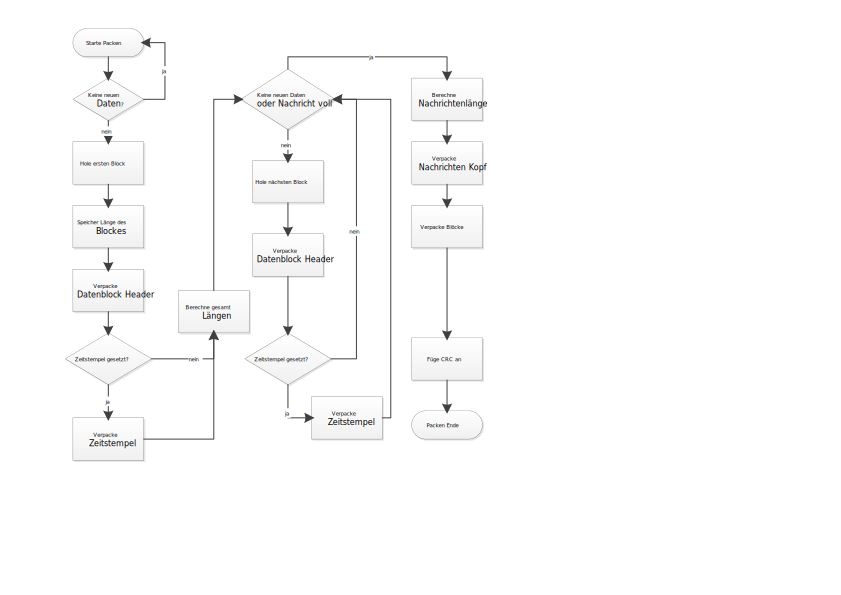
\includegraphics[scale=.5]{AlgorithmusPacketizer.pdf}
\caption{Algorithmus Packetizer}
\label{fig:AlgorithmusPacketizer}
\end{figure}

\subsection{Netzwerk}

Beschreiben der Klasse \Code{UDPSocket} und Erläuterung. Wieso wurde udp
genommen?

\subsection{StoreManager}

Während der Entwicklung des Moduls \Code{Sender} wurde eine weitere Eigenschaft
der Software gefordert.
Die Daten, welchen während des Progammablaufes erstellt und zum Versenden
gespeichert werden, sollen auch nach einem Programmabsturz oder nach einem
Stromausfall noch vorhanden sein. Weil die Klasse \Code{SmartPrioritizedQueue}
die Daten im RAM hinterlegt, wären diese verloren.
Für das Abspeichern der Daten auf die Festplatte existieren prinzipielle drei Methoden.

\begin{enumerate}
\item Jede erzeugte Variable wird direkt auf der Festplatte abgespeichert.
\item Ein Datenpacket (mehrere Variablen) wird an einer Stelle im Programm auf
einmal gespeichert.
\item Es werden Interrupts des Prozessors abgefangen, um Abstürze zu erkennen,
infolgedessen alle wichtigen Daten gesichert werden.
\end{enumerate}

Die erste Methode hat den Vorteil, dass alle Daten sofort gesichert werden und
keine verloren gehen können. Jedoch sind dafür unzählige Festplattenzugriffe
notwendig, wodurch die Laufzeit des Programms stark beeinträchtigt wird. Bei der
dritten Methode sind die Festplattenzugriffe minimal, jedoch können nur
Software- und Hardwarefehler bei der Programmabarbeitung abgefangen werden. Bei
einem Stromausfall würden trotzdem alle Daten verloren gehen. Deshalb wird
Methode Zwei verwendet. Diese stellt den besten Kompromiss aus Datensicherheit
und Performance dar. \newline
Für diese Aufgabe wurde ein Submodul entwickelt, welches die Datenblöcke auf
der Festplatte hinterlegt und bei einem Absturz neu lädt und damit die
\Code{SmartPrioritizedQueue} vorinitialisiert. Dadurch sind die Schnittstellen schon indirekt
vorgegeben, welche das Modul bereitstellen soll. Das ist eine Methode,
welche Datenblöcke auf der Festplatte speichert, eine weitere um diese zu laden
und eine Dritte, mit der bereits gespeicherte Datenblöcke gelöscht werden
können.

\begin{figure}[H]
\centering
\includegraphics[scale=.5]{EinbettungStoreManager.pdf}
\caption{Integration des Submoduls \Code{StoreManager}}
\label{fig:EinbettungStoreManager}
\end{figure}

Die Einbettung des Submoduls \Code{StoreManager} in das Modul \Code{Sender} ist
in \abbildung{EinbettungStoreManager} veranschaulicht. Dazu wird der
\Code{StoreManager} parallel zur \Code{SmartPrioritizedQueue} integriert. Alle
Datenblöcke, welche in die Queue gelangen, werden ebenfalls an die
Klasse \Code{StoreManager} übergeben. Die von dem Submodul \Code{Packetizer}
gelesenen Datenblöcke werden anschliesend wieder gelöscht. Somit ist immer der
aktuelle Datenbestand der \Code{SmartPrioritizedQueue}
zusätzlich auf der Festplatte gesichert. Beim Programmstart wird in der
Initialisierungsmethode des Topmoduls überprüft, ob bereits alte Daten vorhanden
sind, welche anschliessend geladen werden. \newline
Für das Abspeichern der
Daten fehlt noch ein passendes Dateiformat, welches ein schnelles Speichern und
Lesen ermöglicht. Dazu wurden zwei Möglichkeiten gegenüber gestellt. Diese sind
in Tabelle \ref{tab:Speicherformate} aufgeführt.

\begin{longtable}{|lcc|}
\caption{Vergleich der Speicherformate} \\
\hline
\label{tab:Speicherformate}
\textbf{} & \textbf{XML-Datei} & \textbf{Binäre Datei}\\
\hline
  Menschliche Lesbarkeit      &  + & - \\
  Dateigröße      &  0 & + \\
  Geschwindigkeit &  0 & + \\
  Portabilität    &  + & - \\
\hline
\caption*{ + Gut, 0 Medium, - Schlecht }
\end{longtable}
\todo{ QUELLE???????????????????}

Der Tabelle ist zu entnehmen, dass XML auf dem ersten Blick das bessere Format
ist. Dennoch wurde eine binäre Datei verwendet, weil die beiden Schwachstellen
die Portabilität und die Lesbarkeit für einen Menschen für den konkreten
Anwendungsfall keine Bedeutung haben.
Weiterhin soll nur der Computer die Daten auf der Festplatte ablegen und
wieder lesen können Das Versenden über das Internet oder anderen
Medien besitzt damit die Portabilität keinen großen Stellenwert.
Dafür sind die beiden wichtigsten Eigenschaften, die Dateigröße und die
Geschwindigkeit, bei dem Format im Vergleich besser.
\newline
In der Datei werden die folgenden Daten aus dem Datenblock in der
aufgeführten Reihenfolge gespeichert:

\begin{itemize}
\item Datenblockheader 
\item Priorität
\item Zeitstempel
\item Content als ByteArray
\end{itemize}

Aufgrund der Tatsache, dass der Datenblockheader eine Kompression beinhaltet,
und damit die Größe der Variablen unterschiedlich sein kann, wird für die
Variablen festgelegt, dass für jeden Wert die höchste auftretende Bitzahl
aufgerundet zur nächsten Zweierpotenz als Byte verwendet wird. Dadurch
wird das Laden und Speichern stark vereinfacht. Der dabei auftretende zusätzliche
Speicherplatzbedarf kann vernachlässigt werden.
\newline 
Für die Ordnerstruktur wurde eine möglichst flache Hierachie genutzt, welche in
der obersten Stufe den Ordner \Code{Backup} beinhaltet. Darin befinden sich
weitere Ordner, welche als Namen die Nummer des Datentypes beinhalten. In diesem liegen die binären
Dateien dessen Namen aus der Nummer der DOID und der Sequenznummer besteht.
Diese sind durch einen Unterstrich voneinander getrennt. Die drei Parameter
werden von der Methode remove zum Löschen einer Datei übergeben, um diese
eindeutig zu identifizieren.

\section{Modulaufbau Empfänger}

Auf der Empfängerseite sollen die ankommenden Nachrichten empfangen und geparst
werden, um an die darin enthaltenen Informationen zu gelangen. Das Empfangen
durch das Submodul \Code{UDPSocket} ist blockend. Deswegen wird der Vorgang
nebenläufig ausgeführt, damit der Programmablauf nicht behindert wird. Anschliessend wird
die Nachricht geparst und nach dem Beenden des Vorganges ein Callback
\todo{erklären was callback ist} ausgelöst. Bei einem Callback wird
ein Zeiger auf die Speicheradresse der Funktion in der Klasse gespeichert. Durch
Aufruf der Funktion ist es möglich den sequentiellen Programmablauf an einer
anderen Stelle weiterlaufen zu lassen. Nach Abarbeitung dieser kehrt der Ablauf
zur ursprünglichen Position zurück. Diese Funktion kann mittels einer Methode
registriert werden, in der die geparsten Daten weiter verarbeitet werden können.
Die Callbackfunktion könnte beispielsweise die Visualisierung der Daten
übernehmen. \newline 
In \abbildung{BlockdiagrammEmpfaenger} ist eine schematische Darstellung des
Moduls dargestellt. Die Implementierung wird im Folgendem näher erläutert.

\begin{figure}[H]
\centering
\includegraphics[scale=.5]{BlockdiagrammEmpfaenger.pdf}
\caption{Übersicht des Empfängers}
\label{fig:BlockdiagrammEmpfaenger}
\end{figure}

\subsection{Parser}

Der Parser basiert auf dem in Kapitel \ref{sec:ProtokolDesign}
vorgestellten Protokoll-Design.
Anhand dieser Daten wird die empfangende Nachricht Bit für Bit analysiert
und die Informationen herrausgezogen. 
Die Klasse \Code{UDPSocket} empfängt neue Daten und gibt diese an
die Klasse \Code{MessageParser} weiter. Dieser parst den Nachrichtenheader.
Dessen Algorithmus ist in \abbildung{AlgorithmusMessageParser} dargestellt.
Anschließend werden die Datenblockheader geparst. Der Content wird von der
Klasse \Code{DataBlockProcessing} verarbeitet.

\begin{figure}[H]
\centering
\includegraphics[scale=.5]{AlgorithmusMessageParser.pdf}
\caption{Algorithmus zum Parsen der Nachricht}
\label{fig:AlgorithmusMessageParser}
\end{figure}

Dafür wird ein Softwarekonzept namens Policy-Based-Template-Meta Programmierung
\todo{LINK buch + wiki} verwendet, damit die unterschiedlichen Datentypen der
Datenblöcke nach dem Parsen wieder in einem typsicheren Format vorliegen und
einfacher verwendet werden können.
Der Templateklasse werden die folgenden vier Klassen als Templateparameter
Klasse übergeben:

\begin{itemize}
\item T - Datentyp des Rückgabewertes des Parsers
\item Parser - Klasse zum Parsen des Datentypes
\item C - Datentyp der als Callback zurückgegeben wird
\end{itemize}

Der Parameter \Code{Parser} erbt zusätzlich von einer
Schnittstelle gleichen Namens. Die Klasse \Code{DataBlockProcessing} erbt
wiederum von dem Parameter \Code{Parser}.
Dadurch besteht die Möglichkeit in der Klasse auf Funktionen und
Membervariablen zugreifen zu können.
Durch dieses Vorgehen kann das Verhalten der Klasse einfach durch die
Templateparameter verändert werden. Weil der Grundalgorithmus des Parser für
die Datenblöcke für jeden Datentyp identisch ist und lediglich die Art und
Weise verändert werden muss, wie die Daten geparst werden müssen,
ist dieser Weg der optimalste. Durch das Konzept wurden
Redundanzen im Quellcode vermieden und weitere Datentypen lassen sich
sehr einfach hinzufügen ohne bestehenden Quellcode zu verändern. Dadurch konnten
die Grundprinzipien der objektorientierten Programmierung \todo{buch LINK}
eingehalten werden.
Der eben angesprochene Grundalgorithmus ist in Listing 
\ref{lst:PseudocodeDBParser} dargestellt, welcher für jeden Datentyp
durchlaufen wird.

\lstdefinelanguage{pseudo}{
morekeywords={if, else, for, in, remove, from, case, do, forever, to, false,
function, then, end, true, while}, sensitive=true,%
morecomment=[l]\#,%
morestring=[b]',%
}
\lstset{language=pseudo}
\lstset{commentstyle=\textit}
\lstset{literate=
{<=} {$\le$}{2} {!=} {$\neq$}{2} {=} {$\leftarrow$}{2} {==} {=}{2} {&&} {$\cap$}{2} {||} {$\cup$}{2} }
\lstinputlisting[label=lst:PseudocodeDBParser,caption=Pseudocode
des Datenblock Parsers]{Listings/PseudocodeDBParser.txt}
